\section{Casi d'uso}
    \subsection{Attori dei casi d'uso}
    \subsubsection{Attori primari}
    Gli attori che il gruppo ha ritenuto essere i più adeguati sono:
        \begin{itemize}
            \item \textbf{Utente generico:} si divide in:
                \begin{itemize}
                    \item \textbf{Utente non autenticato:} utente che può navigare nell'e-commerce e può usufruire di alcune funzionalità, come la visualizzazione e la ricerca dei prodotti, che può aggiungere al proprio carrello, la applicazione di filtri e categorie per la ricerca, e infine di potersi autenticare.
                    \item \textbf{Utente autenticato:} un utente autenticato può a sua volta essere:
                        \begin{itemize}
                            \item \textbf{Cliente autenticato:} cliente che ha effettuato il login, può accedere a molte funzionalità, come l'aggiunta di prodotti al carrello, l'acquisto, la visualizzazione della lista degli ordini, la possibilità di contattare il venditore;
                            \item \textbf{Venditore autenticato:} venditore che ha effettuato il login, può accedere alle funzionalità relative all'amministrazione dei prodotti e delle categorie.
                        \end{itemize}
                        \begin{figure}[!ht]
                            \caption{Attori primari}
                            \vspace{5px}
                            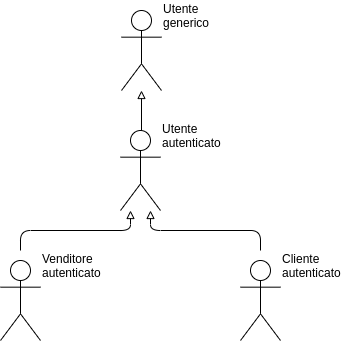
\includegraphics[scale=0.59]{../../../Images/AnalisiRequisiti/attori}
                            \centering
                        \end{figure}
                \end{itemize}
        \end{itemize}
        \subsubsection{Attori secondari}
        \begin{itemize}
            \item \textbf{Amazon Cognito:} servizio esterno per il login e per la gestione delle credenziali;
            \item \textbf{Stripe:} servizio esterno per la gestione dei pagamenti.
        \end{itemize}
        \newpage
    \subsection{Elenco dei casi d'uso}
        \textbf{Utilizzo della piattaforma:}
        \begin{figure}[!ht]
            \caption{Casi d'uso che interessano gli utenti}
            \vspace{10px}
            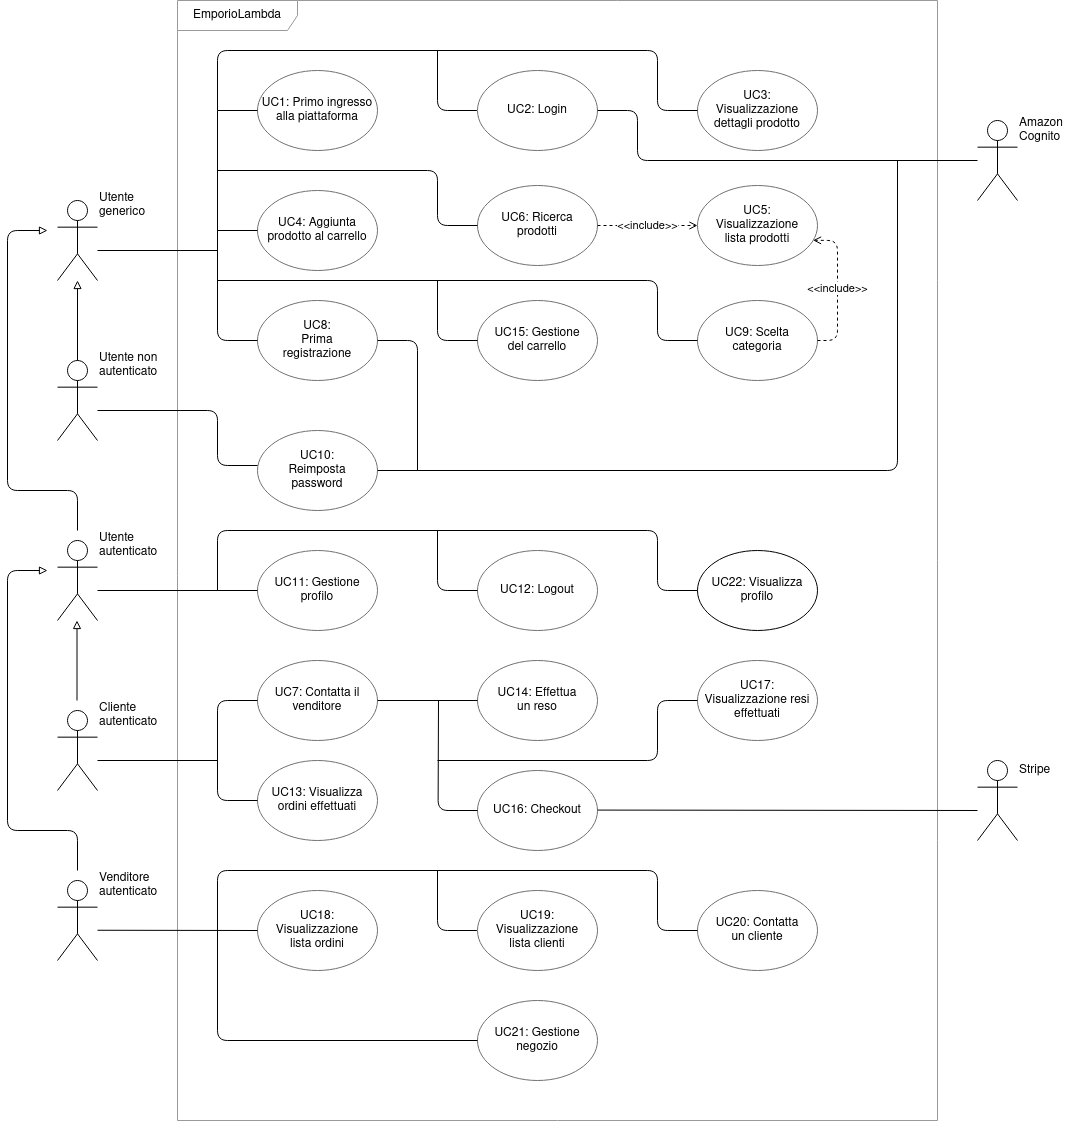
\includegraphics[scale=0.44]{../../../Images/AnalisiRequisiti/casiUso}
            \centering
        \end{figure}
        \subsection{UC1: Primo ingresso alla piattaforma}
        \subsection{UC2: Login}
        \subsection{UC3: visualizzazione dettagli di un prodotto}
        \subsection{UC4: Aggiunta di un prodotto al carrello}
        \subsection{UC5: Ricerca dei prodotti}
        \subsection{UC6: Visualizzazione della lista dei prodotti}
        \subsection{UC7: Contatta il venditore}
        \subsection{UC8: Prima registrazione}
        \subsection{UC9: Scelta della categoria}
        \subsection{UC10: Reimposta password (dimenticata)}
        \subsection{UC11: Gestione credenziali}
        \begin{itemize}
            \item \textbf{Descrizione}
            \item \textbf{Attore Primario}
            \item \textbf{Attore Secondario}
            \item \textbf{Precondizione}
            \item \textbf{Input}
            \item \textbf{Postcondizione}
            \item \textbf{Scenario Principale}
            \item \textbf{Estensioni}
            \item \textbf{Generalizzazioni}
            \item \textbf{Inclusioni}
        \end{itemize}

        
        \subsection{UC12: Logout}
        \begin{itemize}
            \item \textbf{Descrizione:}
            \item \textbf{Attore Primario:}
            \item \textbf{Attore Secondario:}
            \item \textbf{Precondizione:}
            \item \textbf{Input:}
            \item \textbf{Postcondizione:}
            \item \textbf{Scenario Principale:}
            \item \textbf{Estensioni:}
            \item \textbf{Generalizzazioni:}
            \item \textbf{Inclusioni:}
        \end{itemize}


        \subsection{UC13: Gestione degli ordini effettuati}
        \begin{itemize}
            \item \textbf{Descrizione:}
            \item \textbf{Attore Primario:}
            \item \textbf{Attore Secondario:}
            \item \textbf{Precondizione:}
            \item \textbf{Input:}
            \item \textbf{Postcondizione:}
            \item \textbf{Scenario Principale:}
            \item \textbf{Estensioni:}
            \item \textbf{Generalizzazioni:}
            \item \textbf{Inclusioni:}
        \end{itemize}


        \subsection{UC14: Effettua un reso}
        \begin{itemize}
            \item \textbf{Descrizione:}
            \item \textbf{Attore Primario:}
            \item \textbf{Attore Secondario:}
            \item \textbf{Precondizione:}
            \item \textbf{Input:}
            \item \textbf{Postcondizione:}
            \item \textbf{Scenario Principale:}
            \item \textbf{Estensioni:}
            \item \textbf{Generalizzazioni:}
            \item \textbf{Inclusioni:}
        \end{itemize}


        \subsection{UC15: Gestione del carrello}
        \begin{figure}[!ht]
            \caption{Diagramma di UC15: Gestione del carrello}
            \vspace{10px}
            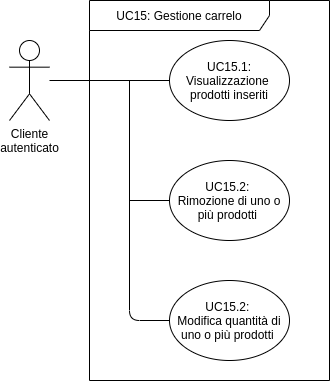
\includegraphics[scale=0.5]{../../../Images/AnalisiRequisiti/UC15}
            \centering
        \end{figure}
        \begin{itemize}
            \item \textbf{Descrizione:} questa sezione tratta l'insieme di operazioni che un utente generico fa per gestire i prodotti nel carrello;
            \item \textbf{Attore Primario:} utente generico;
            \item \textbf{Precondizione:} l'utente si trova in una pagina della piattaforma;
            \item \textbf{Input:} l'utente clicca il bottone per entrare nel carrello;
            \item \textbf{Postcondizione:} l'utente ha completato le operazioni per gestire i prodotti nel carrello;
            \item \textbf{Scenario Principale:}
        \end{itemize}
        \subsubsection{UC15.1: Visualizzazione dei prodotti inseriti}
        \begin{itemize}
            \item \textbf{Descrizione:} sezione per visualizzare tutti i prodotti inseriti nel carrello;
            \item \textbf{Attore Primario:} utente generico;
            \item \textbf{Precondizione:}  l'utente si trova in una pagina della piattaforma;
            \item \textbf{Input:} l'utente clicca il bottone per entrare nel carrello;
            \item \textbf{Postcondizione:} l'utente si trova sulla pagina principale del carrello e vede tutti i prodotti presenti al suo interno;
            \item \textbf{Scenario Principale:}
                \begin{itemize}
                    \item l'utente si trova in una pagina della piattaforma;
                    \item l'utente clicca il bottone per entrare nel carrello;
                    \item una volta entrato l'elenco dei prodotti è subito visibile.
                \end{itemize}
        \end{itemize}
        \subsubsection{UC15.2: Rimozione di uno o più prodotti}
        \begin{itemize}
            \item \textbf{Descrizione:} sezione per rimuovere uno o più prodotti dal carrello;
            \item \textbf{Attore Primario:} utente generico;
            \item \textbf{Precondizione:} l'utente è nella pagina del carrello (UC15.1);
            \item \textbf{Input:} l'utente seleziona i prodotti da rimuovere dal carrello;
            \item \textbf{Postcondizione:} vengono rimossi i prodotti selezionati;
        \end{itemize}
        \subsubsection{UC15.3: Modifica della quantità di uno o più prodotti}
        \begin{itemize}
            \item \textbf{Descrizione:} sezione per modificare le quantità dei prodotti nel carrello;
            \item \textbf{Attore Primario:} utente generico;
            \item \textbf{Precondizione:} l'utente è nella pagina del carrello (UC15.1);
            \item \textbf{Input:} l'utente inserisce le modifiche desiderate ai prodotti;
            \item \textbf{Postcondizione:} le modifiche sono applicate;
            \item \textbf{Estensioni:} 
                \begin{itemize}
                    \item se la nuova quantità non dovesse essere disponibile per il venditore, l'utente viene avvisato.
                \end{itemize}
        \end{itemize}

        
        \subsection{UC16: Checkout}
            \begin{figure}[!ht]
                \caption{Diagramma di UC16: Checkout}
                \vspace{10px}
                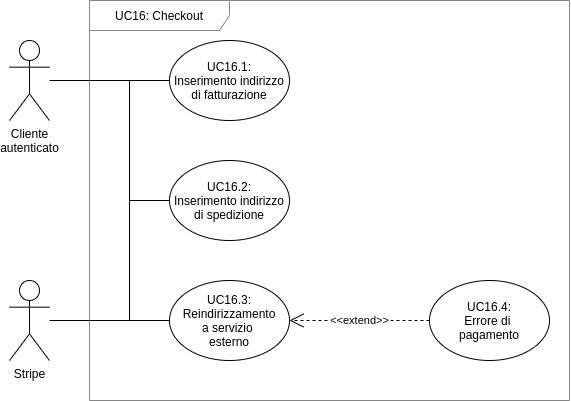
\includegraphics[scale=0.5]{../../../Images/AnalisiRequisiti/UC16}
                \centering
            \end{figure}
                \begin{itemize}
                \item \textbf{Descrizione:} caso d'uso per la creazione di un nuovo ordine e l'acquisto dei prodotti inseriti nel carrello;
                \item \textbf{Attore Primario:} cliente autenticato;
                \item \textbf{Attore Secondario:} Stripe, gestore di pagamenti di terze parti;
                \item \textbf{Precondizione:} il cliente si trova sul carrello e ha già inserito almeno un prodotto;
                \item \textbf{Input:} il cliente clicca il bottone per iniziare il checkout;
                \item \textbf{Postcondizione:} l'ordine viene emesso e aggiunto alla lista degli ordini di quel cliente; i prodotti acquistati vengono rimossi dal carrello e viene diminuita la quantità dal deposito del venditore;
                \item \textbf{Scenario Principale:} 
                    \begin{itemize}
                        \item il cliente preme sul pulsante per entrare nella sezione del checkout;
                        \item il cliente inserisce i dati di fatturazione (UC16.1) e, se diversi, i dati di spedizione (UC16.2);
                        \item vengono inseriti eventuali costi di spedizione;
                        \item il cliente viene reindirizzato al servizio di pagamento esterno, dove inserisce i dati di pagamento;
                        \item l'ordine è emesso e segnato come completato.
                    \end{itemize}
                \item \textbf{Estensioni:}
                    \begin{itemize}
                        \item se il cliente decide di non completare il checkout, può uscire dalla pagina senza causare modifiche al carrello;
                        \item se il pagamento ha avuto esito negativo, l'ordine non viene emesso e quindi è necessario ricominciare il pagamento.
                    \end{itemize}
            \end{itemize}
            \subsubsection{UC16.1: Inserimento dell'indirizzo di fatturazione}
                \begin{itemize}
                    \item \textbf{Descrizione:} Sezione per l'inserimento dell'indirizzo fatturazione;
                    \item \textbf{Attore Primario:} cliente autenticato;
                    \item \textbf{Precondizione:} il cliente si trova nella fase di checkout;
                    \item \textbf{Input:} il cliente inserisce i dati richiesti dalla pagina;
                    \item \textbf{Postcondizione:} si procede con la fase successiva del checkout (UC16.2)
                    \item \textbf{Scenario Principale:} il cliente inserisce negli appositi spazi i dati per completare l'indirizzo di fatturazione.
                \end{itemize}
            \subsubsection{UC16.2: Inserimento dell'indirizzo di spedizione}
                \begin{itemize}
                    \item \textbf{Descrizione:} Sezione per l'inserimento dell'indirizzo spedizione;
                    \item \textbf{Attore Primario:} cliente autenticato;
                    \item \textbf{Precondizione:} il cliente si trova nella fase di checkout;
                    \item \textbf{Input:} il cliente inserisce i dati richiesti dalla pagina, oppure clicca un pulsante se l'indirizzo di spedizione è lo stesso di quello di fatturazione;
                    \item \textbf{Postcondizione:} si procede con la fase successiva del checkout (UC16.3)
                    \item \textbf{Scenario Principale:} il cliente inserisce negli appositi spazi i dati per completare l'indirizzo di spedizione oppure clicca il pulsante per autocompletarli se è il medesimo di quello di fatturazione.
                \end{itemize}
            \subsubsection{UC16.3: Reindirizzamento al servizio di pagamento esterno}
                \begin{itemize}
                    \item \textbf{Descrizione:} Sezione per il pagamento dell'ordine da effettuare;
                    \item \textbf{Attore Primario:} cliente autenticato;
                    \item \textbf{Attore Secondario:} Stripe, gestore di pagamenti di terze parti;
                    \item \textbf{Precondizione:} il cliente ha inserito i dati per la fatturazione e la spedizione nella sezione del checkout;
                    \item \textbf{Input:} il cliente preme il pulsante per il pagamento;
                    \item \textbf{Postcondizione:} il pagamento ha avuto esito positivo, l'ordine viene confermato e viene decrementata la quantità dei prodotti disponibili al venditore, in base al numero di prodotti acquistati dal cliente;
                    \item \textbf{Scenario Principale:}
                    \item \begin{itemize}
                        \item il cliente preme sul pulsante e viene reindirizzato al servizio esterno per eseguire il pagamento;
                        \item il cliente inserisce i propri dati ed esegue il pagamento;
                        \item il pagamento è riuscito e l'ordine viene confermato.
                    \end{itemize}
                    \item \textbf{Estensioni:}
                    \begin{itemize}
                        \item il pagamento non è riuscito, viene visualizzato un errore di pagamento (UC16.4) e si viene reindirizzati alla pagina del checkout per riprovare.
                    \end{itemize}
                \end{itemize}
            \subsubsection{UC16.4: Errore di pagamento}
                \begin{itemize}
                    \item \textbf{Descrizione:} visualizzazione di un errore per un fallimento nella fase di pagamento;
                    \item \textbf{Attore Primario:} Stripe
                    \item \textbf{Precondizione:} il cliente ha inserito i dati del pagamento;
                    \item \textbf{Input:} Stripe ritorna un errore nel risultato del pagamento;
                    \item \textbf{Postcondizione:} viene visualizzato un messaggio di errore, successivamente il cliente viene reindirizzato alla sezione del checkout;
                \end{itemize}

        \subsection{UC17: Visualizzazione dei resi effettuati}
            \begin{itemize}
                \item \textbf{Descrizione:}
                \item \textbf{Attore Primario:}
                \item \textbf{Attore Secondario:}
                \item \textbf{Precondizione:}
                \item \textbf{Input:}
                \item \textbf{Postcondizione:}
                \item \textbf{Scenario Principale:}
                \item \textbf{Estensioni:}
                \item \textbf{Generalizzazioni:}
                \item \textbf{Inclusioni:}
            \end{itemize}
        \subsection{UC18: Visualizzazione della lista degli ordini}
        \begin{itemize}
            \item \textbf{Descrizione:}
            \item \textbf{Attore Primario:}
            \item \textbf{Attore Secondario:}
            \item \textbf{Precondizione:}
            \item \textbf{Input:}
            \item \textbf{Postcondizione:}
            \item \textbf{Scenario Principale:}
            \item \textbf{Estensioni:}
            \item \textbf{Generalizzazioni:}
            \item \textbf{Inclusioni:}
        \end{itemize}
        \subsection{UC19: Visualizzazione della lista degli utenti}
            \begin{itemize}
                \item \textbf{Descrizione:}
                \item \textbf{Attore Primario:}
                \item \textbf{Attore Secondario:}
                \item \textbf{Precondizione:}
                \item \textbf{Input:}
                \item \textbf{Postcondizione:}
                \item \textbf{Scenario Principale:}
                \item \textbf{Estensioni:}
                \item \textbf{Generalizzazioni:}
                \item \textbf{Inclusioni:}
            \end{itemize}
        \subsection{UC20: Contatta un cliente}
        \begin{itemize}
            \item \textbf{Descrizione}
            \item \textbf{Attore Primario}
            \item \textbf{Attore Secondario}
            \item \textbf{Precondizione}
            \item \textbf{Input}
            \item \textbf{Postcondizione}
            \item \textbf{Scenario Principale}
            \item \textbf{Estensioni}
            \item \textbf{Generalizzazioni}
            \item \textbf{Inclusioni}
        \end{itemize}
        \subsection{UC21: Gestione del negozio}
        \begin{itemize}
            \item \textbf{Descrizione}
            \item \textbf{Attore Primario}
            \item \textbf{Attore Secondario}
            \item \textbf{Precondizione}
            \item \textbf{Input}
            \item \textbf{Postcondizione}
            \item \textbf{Scenario Principale}
            \item \textbf{Estensioni}
            \item \textbf{Generalizzazioni}
            \item \textbf{Inclusioni}
        \end{itemize}

